%%%%%%%%%%%%%%%%%%%%%%%%%
% Dokumentinformationen %
%%%%%%%%%%%%%%%%%%%%%%%%%
\newcommand{\titleinfo}{Physik 1 - Zusammenfassung}
\newcommand{\authorinfo}{C. v./d.G.}
\newcommand{\versioninfo}{$Rev: 1.0 $ | 
						gem\"ass Unterricht HS2017}

%%%%%%%%%%%%%%%%%%%%%%%%%%%%%%%%%%%%%%%%%%%%%
% Standard projektübergreifender Header für
% - Makros 
% - Farben
% - Mathematische Operatoren
%
% DORT NUR ERGÄNZEN, NICHTS LÖSCHEN
%%%%%%%%%%%%%%%%%%%%%%%%%%%%%%%%%%%%%%%%%%%%%

%%% Open Tasks %%%

% - Skilift-Skizze & Formeln
% - 

%%%%%%%%%%%%%%%%%%%


% Genereller Header
\documentclass[10pt,twoside,a4paper,fleqn]{article}
% Dateiencoding
\usepackage[utf8]{inputenc}
% Seitenränder
\usepackage[left=1cm,right=1cm,top=1cm,bottom=1cm,includeheadfoot]{geometry}
% Sprachpaket
\usepackage[ngerman]{babel,varioref}

% Pakete
\usepackage{amssymb,amsmath,fancybox,graphicx,lastpage,wrapfig,fancyhdr,hyperref,verbatim,floatflt,multicol,multirow,rotating,pdflscape,array,longtable,listings}

% Zum Bilder einfach in Tabellen einfügen (valign=t)
\usepackage[export]{adjustbox}

%%%%%%%%%%%%%%%%%%%%
% Generelle Makros %
%%%%%%%%%%%%%%%%%%%%
\newcommand{\skript}[1]{$_{\textcolor{red}{\mbox{\small{Skript S.#1}}}}$}
\newcommand{\verweis}[2]{\small{(siehe auch \ref{#1}, #2 (S. \pageref{#1}))}}
\newcommand{\verweiskurz}[1]{(\small{siehe \ref{#1}\normalsize)}}
\newcommand{\subsubadd}[1]{\textcolor{black}{\mbox{#1}}}
\newcommand{\formelbuch}[1]{$_{\textcolor{red}{\mbox{\small{S#1}}}}$}

\newcommand{\kuchling}[1]{$_{\textcolor{red}{\mbox{\small{Kuchling #1}}}}$}
\newcommand{\stoecker}[1]{$_{\textcolor{orange}{\mbox{\small{Stöcker #1}}}}$}
\newcommand{\sachs}[1]{$_{\textcolor{blue}{\mbox{\small{Sachs S. #1}}}}$}
\newcommand{\hartl}[1]{$_{\textcolor{green}{\mbox{\small{Hartl S. #1}}}}$}

\newcommand{\schaum}[1]{\tiny Schaum S. #1}

\newcommand{\skriptsection}[2]{\section{#1 {\tiny Skript S. #2}}}
\newcommand{\skriptsubsection}[2]{\subsection{#1 {\tiny Skript S. #2}}}
\newcommand{\skriptsubsubsection}[2]{\subsubsection{#1 {\tiny Skript S. #2}}}

\newcommand{\matlab}[1]{\footnotesize{(Matlab: \texttt{#1})}\normalsize{}}

%%%%%%%%%%
% Farben %
%%%%%%%%%%
\usepackage{xcolor}

%%%%%%%%%%%%%%%%%%%%%%%%%%%%
% Mathematische Operatoren %
%%%%%%%%%%%%%%%%%%%%%%%%%%%%
\DeclareMathOperator{\sinc}{sinc}
\DeclareMathOperator{\sgn}{sgn}
\DeclareMathOperator{\Real}{Re}
\DeclareMathOperator{\Imag}{Im}
%\DeclareMathOperator{\e}{e}
\DeclareMathOperator{\cov}{cov}
\DeclareMathOperator{\PolyGrad}{PolyGrad}

%Makro für 'd' von Integral- und Differentialgleichungen 
\newcommand*{\diff}{\mathop{}\!\mathrm{d}}


%%%%%%%%%%%%%%%%%%%%%%%%%%%
% Fouriertransformationen %
%%%%%%%%%%%%%%%%%%%%%%%%%%%
\usepackage{trfsigns, trsym}
%\unitlength1cm
% Zeitbereich -- Frequenzbereich
%\newcommand{\laplace}
%{
%\begin{picture}(1,0.5)
%\put(0.2,0.1){\circle{0.14}}\put(0.27,0.1){\line(1,0){0.5}}\put(0.77,0.1){\circle*{0.14}}
%\end{picture}
%}
% Frequenzbereich -- Zeitbereich
%\newcommand{\Laplace}
%{
%\begin{picture}(1,0.5)
%\put(0.2,0.1){\circle*{0.14}}\put(0.27,0.1){\line(1,0){0.45}}\put(0.77,0.1){\circle{0.14}}
%\end{picture}
%}


% Fouriertransformationen
\unitlength1cm
\newcommand{\FT}
{
\begin{picture}(1,0.5)
\put(0.2,0.1){\circle{0.14}}\put(0.27,0.1){\line(1,0){0.5}}\put(0.77,0.1){\circle*{0.14}}
\end{picture}
}


\newcommand{\IFT}
{
\begin{picture}(1,0.5)
\put(0.2,0.1){\circle*{0.14}}\put(0.27,0.1){\line(1,0){0.45}}\put(0.77,0.1){\circle{0.14}}
\end{picture}
}




%%%%%%%%%%%%%%%%%%%%%%%%%%%%
% Allgemeine Einstellungen %
%%%%%%%%%%%%%%%%%%%%%%%%%%%%
%PDF Info
\hypersetup{pdfauthor={\authorinfo},pdftitle={\titleinfo},colorlinks=false}
\author{\authorinfo}
\title{\titleinfo}

%%%%%%%%%%%%%%%%%%%%%%%
% Kopf- und Fusszeile %
%%%%%%%%%%%%%%%%%%%%%%%
\pagestyle{fancy}
\fancyhf{}
%Linien oben und unten
\renewcommand{\headrulewidth}{0.5pt} 
\renewcommand{\footrulewidth}{0.5pt}

\fancyhead[L]{\titleinfo{ }\tiny{(\versioninfo)}}
%Kopfzeile rechts bzw. aussen
\fancyhead[R]{Seite \thepage { }von \pageref{LastPage}}
%Fusszeile links bzw. innen
\fancyfoot[L]{\footnotesize{\authorinfo}}
%Fusszeile rechts bzw. ausen
\fancyfoot[R]{\footnotesize{\today}}
% Lizenz CC-BY-NC-SA
% Headerfile für die Einbindung einer Lizenzgrafik in den Footer
% Verwendung: \lizenz{cc-by-nc-sa}{small}
\newcommand{\lizenz}[2]
{
\fancyfoot[C]{
  \includegraphics[width=1.6cm]{./header/lizenzen/#1/#2.png}
}
}
\lizenz{cc-by-nc-sa}{small}
% Einrücken verhindern versuchen
\setlength{\parindent}{0pt}

% Zeilenhöhe Tabellen:
\newcommand{\arraystretchOriginal}{1.5}
\renewcommand{\arraystretch}{\arraystretchOriginal}


\usepackage{tikz}

% Möglichst keine Ergänzungen hier, sondern in header.tex
\begin{document}

% Einleitung
\section{Physik 1: Mechanik}

\subsection{Was sind Kräfte?}
Die Kraft ist einer der physikalischen Grundbegriffe, die streng genommen nicht 
definiert, sondern nur durch ihre Wirkung beschrieben werden können:
\begin{itemize}
\item Dynamische Wirkung: Eine Kraft kann den Bewegungszustand eines Körpers ändern.
\item Statische Wirkung: Eine Kraft kann eine Deformation eines Körpers bewirken (Körper bleibt aber in Ruhe).
\end{itemize}

$\lbrack F \rbrack =  N = \frac{kg \cdot m}{s^2}$

\subsection{Fundamentalkräfte}
\begin{itemize}
	\item Schwerkraft
	\item Elektrische Kraft
	\item Kernkräfte (Schwache \& Starke Kraft)
\end{itemize}

\subsection{Fragen}
\begin{enumerate}
	\item Wann müssen Sie das Modell des Starren Körpers benützen? \\
	\item Welche elastischen Konstanten kennen Sie?
	\item Was ist der Unterschied zwischen dem Torsionsmodul und 
	dem Gleitmodul?
\end{enumerate}

%Statik
\section{Statik}

\begin{multicols}{2}
\textbf{Generelles Vorgehen} \\
1. Skizze mit allen Kräften aufzeichnen \\
2. Koordinatensystem einführen \\
3. Falls nötig, Drehpunkt von Drehmoment einführen \\
4. Gleichgewichtsbedingungs-/ Gleichungssystem aufstellen \\
5. Gleichungssystem auflösen \\
\columnbreak
\\
\textbf{Gleichgewichtsbedingung starrer Körper} \\
Ein Körper ist dann im Gleichgewicht, wenn keine resultierende Kraft auf ihn wirkt, d.h. die Summe der ihn angreifenden Kräfte ist null. \\
$\sum\limits_{i=0}^{n} F_{ix} = 0,  \; \sum\limits_{i=0}^{n} F_{iy} = 0, \; \sum\limits_{i=0}^{n} F_{iz} = 0 $
\end{multicols}

\subsection{Starrer Körper - Statik des Massenpunktes}
Ein Massenpunkt ist ein Körper, dessen ganze Masse in 
einem Punkt konzentriert ist. \\
Ein starrer Körper wird durch die an ihm angreifenden 
Kräfte nicht deformiert. Die Gerade, die durch den Angriffspunkt einer Kraft F geht und 
deren Richtung durch die Richtung von F bestimmt ist, wird 
Wirkungslinie von  F genannt. Für starre Körper gilt nun 
folgender Satz:
\textit{In einem starren Körper kann eine Kraft entlang ihrer 
Wirkungslinie beliebig verschoben werden, ohne dass sich 
an ihrer Wirkung etwas ändert.} 



\subsubsection{Kontaktkraft}
Bezeichnet die Kraft eines auf einer Oberfläche liegenden Körpers, die der Schwerkraft entgegenwirkt. Sie steht immer im rechten Winkel zur Ebene und zur Reibungskraft $F_R$. \\


\subsubsection{Reibung \& Gleitreibung}
\begin{minipage}{15.5cm}
Reibungskraft $F_{R} = \mu_{H} \cdot F_{N}$ (Der Körper haftet noch immer am Untergrund)\\
Gleitreibungskraft $F_G =  \mu_{G} \cdot F_{N}$ (Der Körper bewegt sich) \\
Achtung: Bei Schiefen Ebenen entspricht $F_{N}$ nicht $F_{G}$ \\
Die Reibungskraft ist nicht von der Grösse der Kontaktfläche abhängig, sondern nur vom Gewicht. \\
Die Reibungskraft geht immer in die Gegenrichtung der Zugkraft und ist im rechten Winkel zu $F_{N}$.
\end{minipage}
\begin{minipage}{4cm}
	\adjustbox{width=3cm}{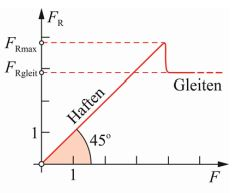
\includegraphics{bilder/reibungs}}
\end{minipage}


\subsubsection{Drehmoment}
\begin{minipage}{15cm}
Zwei entgegengesetzt gerichtete gleich grosse Kräfte mit 
parallelen, aber verschiedenen Wirkungslinien bilden ein 
Kräftepaar. Dies ergibt eine DREHWIRKUNG.
Eine drehende Wirkung lässt sich mit einem Kräftepaar oder, 
bezüglich eines Bezugspunktes, mit einer Einzelkraft erzielen.
Das Drehmoment eines Kräftepaars ist das Produkt des Betrags der Kraft und des Abstands der Wirkungslinien. \\
$M = a \cdot F$ , a ist der Abstand zum Drehpunkt \\
Drehmoment als Vektor im Raum: $\overrightarrow{M} = \overrightarrow{r} \times \overrightarrow{F} = F \cdot r \cdot \sin(\alpha)$ \\
 $\overrightarrow{M}$ steht im rechten Winkel auf der Ebene $\overrightarrow{r},  \overrightarrow{F}$ \\
Der Drehsinn ist in Gegenuhrzeigersinn. \\
\textbf{Tipp:} Der Bezugspunkt zu einem Drehmoment kann beliebig gewählt werden. Besonders geeignet sind Bezugspunkte, wo andere Kräfte Null ergeben!.  
\end{minipage}
\begin{minipage}{4cm}
\adjustbox{width=3cm}{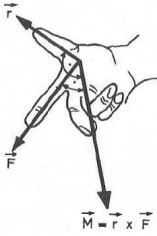
\includegraphics{bilder/drehmoment_2}}
\end{minipage}

\subsubsection{Schwerpunkt}
Der Schwerpunkt S eines Körpers ist der Punkt, in dem der unter der Wirkung der Schwerkraft stehende Körper unterstützt oder aufgehängt werden muss, damit er im Gleichgewicht ist. Der ausgedehnte Körper kann im Bezug auf die Schwerkraft durch einen Massenpunkt ersetzt werden. Eine Kraft auf den Schwerpunkt eines Körpers erzeugt kein Drehmoment (Abstand zum Drehpunkt ist Null)! \\
$ x_s = \frac{\Sigma_{i} x_{i} \cdot m_{i}}{\Sigma_{i} m_{i}}$
$ y_s = \frac{\Sigma_{i} y_{i} \cdot m_{i}}{\Sigma_{i} m_{i}}$
$ z_s = \frac{\Sigma_{i} z_{i} \cdot m_{i}}{\Sigma_{i} m_{i}}$ \\
Schwerpunkt eines Halbkreises: $x = 0,s \; y = \frac{4r}{3\pi}$ \\


\subsection{Deformierbare Körper}
- Elastisches Verhalten: Metalle, Keramik \\
- Plastisches  Verhalten: Plastilin, Knetmasse, Kunststoffe $\overrightarrow{}$ Mikroskopisches Modell mit Versetzung \\
- Moderne Materialien

\begin{multicols}{2}
\subsubsection{Spannung}
Die Kraft F kann in eine zur Fläche A senkrechte Konstante $F_{\perp}$ und eine zur Fläche parallele Konstante $F_{||}$ zerlegt werden.  \\
$\omega = \frac{F_{\perp}}{A} \; \; \tau = \frac{F_{||}}{A}$

\subsubsection{Dehnung / Längenkontraktion}
 Längenänderung $\Delta l:  \sim F / l / \frac{1}{A}$ \\
 Relative Verlängerung: $\frac{\Delta l}{l} = \varepsilon$ \\
Hookesche Gesetz: $ \varepsilon = \frac{1}{E} \cdot \sigma $ \\
Elastizitätsmodul E: \lbrack$ \frac{N}{m^2}$ \rbrack

\subsubsection{Kompression}

Volumenreduktion / Volumen: $\frac{\Delta V}{V} = - \kappa \Delta p$\\
Druckänderung: $\Delta$ p, \\
Kompressibilität $\kappa = \frac{3(1-2\mu)}{E}$


\subsubsection{Querkontraktion / Querdehnung}
Bei einer Längsdehnung eines Stabes tritt auch eine Querkontraktion auf, d.h. der Stab wird dünner. \\
$ \varepsilon_{q} = \frac{\Delta d}{d}$ d ist die Dicke, $\Delta d$ die Änderung der Dicke des Stabes \\
$\varepsilon_{q} = -\mu \varepsilon $ \\
Possionzahl $\mu$ ist zw. 0.15 und 0.5. 

\subsubsection{Schraubenfeder}
$F = c \Delta l, \;$ \\
Federkonstante $c = \frac{Gr^4}{4nR^3}$ \\
r = Drahtradius, n = Anz. Windungen, R = Windungsradius

\subsubsection{Schubbeanspruchung}
%\adjustbox{width=4.5cm}{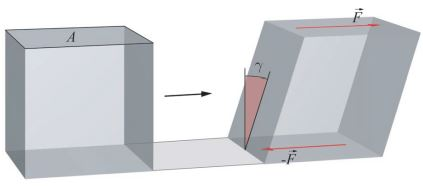
\includegraphics{bilder/schubbeanspruchung}}
$\gamma = \frac{1}{G}\tau$ \\
Schub-/Gleit-/Torsionsmodul G: $\frac{E}{2(1+\mu)} \lbrack \frac{N}{m^2} \rbrack$
\end{multicols}

\begin{multicols}{3}
\textbf{Torsionsfeder} \\
$M = c* \cdot \varphi$ \\
$c = \frac{\varphi G r^4}{2l} $
\columnbreak
\\
\textbf{Balken-Biegung} \\
$z = \frac{4l^3}{Ebh^3}F$ \\
b = Balkenbreite \\
\columnbreak
\\
\textbf{Skalierungsgesetz} \\
$z = \frac{5 \rho g l^4}{32Eh^2}$ \\
h = Höhe des Querschnitts
\end{multicols}



%Kinematik

\section{Kinematik}

Beschreibt Bewegungen von Massenpunkten und 
Körpern, ohne dabei nach den wirkenden Kräften zu 
fragen.
Ein Körper kann sich auf zwei Arten bewegen: 
\begin{itemize}
	\item Translation: Der Körper wird verschoben
	\item Rotation: Der Körper wird gedreht
\end{itemize}

\subsubsection{Geschwindigkeit}
Geschwindigkeit entspricht der pro Zeiteinheit zurückgelegte Wegstrecke \\
Geschwindigkeit: $v = \frac{x_{2} - x_{1}}{t_{2} - t_{1}} = \frac{\Delta s}{\Delta t}$  $v:= [m/s]$ \\

Mittlere Geschwindigkeit: $ \bar{v} = \frac{x(t + \Delta t) - x(t)}{\Delta t}$  $v = \lim_{t \rightarrow 0} \frac{\Delta x}{\Delta t}$

\subsubsection{Beschleunigung}
Die Beschleunigung entspricht der Änderung der Geschwindigkeit pro Zeiteinheit. \\
Mittlere Beschleunigung: $\bar{a} = \frac{\Delta v}{ \Delta t} $   $a:= [m/s^2]$


\subsection{Bewegungen}
\textbf{Tipp:} Immer in $\frac{m}{s}$ rechnen (d.h. $\frac{Wert \; in \; km}{3.6}$, 	Bremsen: $\alpha < 0$ !
\begin{multicols}{3}
	\subsubsection{Gleichförmige B.}
	Konstante Geschwindigkeit: \\
	Reibungskraft entspricht der \\
	Motorenleistung. \\
	$a = 0$ \\
	$v = konstant$\\
	$s = vt + s_0$ \\
	\\
	\\
	\adjustbox{width=5cm}{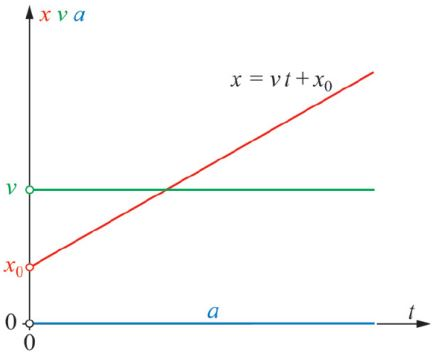
\includegraphics{bilder/gleichfBeschl}}
\columnbreak
	\subsubsection{Gleichmässig beschl. B.}
	$a = konstant$ \\
	$v = \alpha t + v_{0} = \dot s = s'(t)$ \\
	$s = \frac{a}{2}t^2 + v_{0}t + s_{0} = \frac{v_{1}^2 - v_{0}^2}{2a}$ \\
	$a = \frac{v_{1}^2 - v_{0}^2}{2s} = \frac{\Delta v}{\Delta t} = \dot v = s''(t)$ \\
	$v_{2} = \sqrt{v_{0}^2 + 2as}$ \\
	\\
	\\
	\adjustbox{width=5cm}{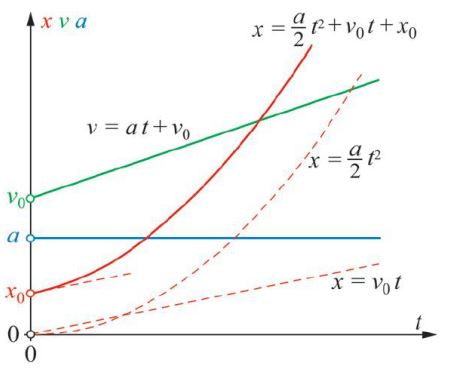
\includegraphics{bilder/gleichmBeschl}}
\columnbreak
	\subsubsection{Benötigte Werte}
	$s_{0}:= Anfangsstrecke$ \\
	$v_{0}:= Startgeschwindigkeit$ \\
	$v_{1}:= Endgeschwindigkeit$ \\
	$\alpha:= Winkelbeschleunigung \; [\frac{rad}{s^2}]$ \\
	$\omega:= Winkelgeschwindigkeit \; [\frac{rad}{s}]$ \\
	$\varphi:= Winkel \; [rad]$ \\
	$T:= Periode $\\
	$f:= Frequenz $\\
	$\omega_{0} := Startwinkelgeschwindigkeit $ \\
	$\omega_{1} := Endwinkelgeschwindigkeit $ \\
	$\varphi_{0} := Startwinkel $ \\
	$a_{z} := Zentralbeschleunigung$ \\
	$n := Drehzahl$ \\
	\\
	$ \omega := 2 \pi n = 2 \pi f$ \\
	$ n:= f = \frac{1}{T} = \frac{1}{\frac{2 \pi}{\omega_0}} = \frac{\omega_o}{2\pi}$
\end{multicols}
	
\subsection{Kreisbewegung}

\begin{multicols}{3}
	\subsubsection{Gleichf"ormige}
	$a = 0 \\
	s = r\varphi \\
	v = r\omega \\
	\omega = \dot \varphi = \frac{v}{r} = 2\pi f\\
	\varphi = \omega t \\
	f = \frac{1}{T} \\
	\overrightarrow{v} = \overrightarrow{\omega} \times \overrightarrow{r}$ \\
	\\
	\\
	\\
	\columnbreak
\subsubsection{Gleichf"ormig beschl.}
	$\alpha = konstant = \dot \omega = \varphi''(t) \\
	a = r \alpha \\
	\omega = \alpha t + \omega_{0} = \sqrt{\omega_{0}^2 + 2 \alpha(\varphi - \varphi_{0})}$ \\
	$\varphi =\frac{a}{2}t^2 + \omega_{0}t + \phi_{0} = \frac{\omega_{1}^2 -\omega_{0}^2}{2a}$	\\
	\adjustbox{width=2.5cm}{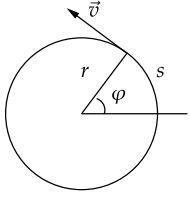
\includegraphics{bilder/gleichfKreis_k}}
	\columnbreak
	\subsubsection{Zentripetalbeschleunigung}
	$\alpha_{z} = \frac{v^2}{r} = r\omega^2 \\
	v = \frac{2\pi r}{T} \\
	F_{z} = ma_{z} = \frac{mv^2}{r} = m\omega^2r$ \\
	\\
	\adjustbox{width=2.5cm}{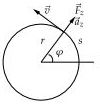
\includegraphics{bilder/zentripetal_k}}
\end{multicols}


	\subsection{Wurfbahnen}
	
	\begin{multicols}{3}
		\subsubsection{Freier Fall}
		$a_{y} = -g \\
		v_{y} = -gt \\
		v_{e} = \sqrt{2gh} \\
		y(t) = -\frac{g}{2}t^2 \\
		t = \sqrt{\frac{2h}{g}}$ \\
		\\
		\\
		\\
		\adjustbox{width=1cm}{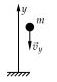
\includegraphics{bilder/hwurf_k}}
	
		\columnbreak
		\subsubsection{Senkrechter Wurf}
		$t_{s} = \lvert{\frac{v_{0}}{g}}\rvert$ \\
		$y(t) = -\frac{g}{2}t^2 + v_0 \cdot t + y_0 $\\
		$h = \frac{v_{0}t}{2} = \lvert{\frac{v_{0}^2}{2g}}\rvert \\
		t_{f} = 2t_{s}$ \\
		$t_{f}:= Flugzeit \\
		t_{s}:= Steigzeit$ \\
		\\
		\adjustbox{width=1cm}{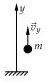
\includegraphics{bilder/hwurf_k3}}
	
		\columnbreak
		\subsubsection{Horizontaler Wurf}
		$a_{x} = 0 \rightarrow{} v_{x} = v_{0}$ Gleichförmige Bew. \\
		$s_{x} = v_{0}t = \sqrt{\frac{2v_{0}^2y}{g}}$ \\
		$a_{y} = -g \rightarrow{} v_{y} = -gt$ Gleichm. beschl.\\
		$y(t) = s_{y} = -\frac{g}{2}t^2 = -\frac{g}{2v_{0}^2}s_{x}^2$ \\
		$t_{F} = \sqrt{\frac{s \cdot h}{g}}$ , $v_{Ges} = \sqrt{v_{x}^2 + v_{y}^2} $ \\
		Parabelgleichung:\\
		\adjustbox{width=2.5cm}{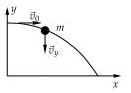
\includegraphics{bilder/hwurf_k2}}
	\end{multicols}
	
	\subsubsection{Schiefer Wurf}
\begin{multicols}{3}
	Gleichförmig in x-Richtung \\
	$a_{x} = 0$ \\
	$v_{x} = v_{0x} = v_0 \cdot \cos(\phi)$ \\
	$v(t)= v_{0x} \cdot t $\\
	\\
	\adjustbox{width=2.5cm}{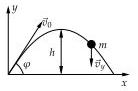
\includegraphics{bilder/schief_k}}
\columnbreak
	\\
	Gleichmässig in y-Richtung \\
	$a_{y} = -g$ (nimmt immer ab)\\
	$v_{y} = v_{oy} - g \cdot t = v_0 \cdot \sin(\phi) - g \cdot t $ \\
	$v(t) = -\frac{1}{2} \cdot a \cdot t^2 + v_{0y} \cdot t + 0$ \\
	$d = \frac{v_{0}^2}{g} \cdot \sin{(2\varphi)} \\$
	$h = \frac{v_{0}^2}{2g}\sin^2{\varphi}$ \\
	$t = \frac{2v_{0} \cdot \sin{\varphi}}{g}$ \\
\columnbreak
\\
	$\Delta y = v_{0}\sin{\varphi}t - \frac{gt^2}{2}$ \\
	$\Delta y = v_{0}\cos{\varphi}t$ \\
	Max. Wurfweite: $x_{Wurf} = \frac{\sin2\alpha \cdot v_{0}^2}{g} \overrightarrow{}$ \\ $\sin2\alpha = 1 \; \overrightarrow{} \alpha = 45^\circ$ \\
	Spez. Wurfweite: $\alpha < 45^\circ \; (Flachwurf)$ \\
	$ \alpha > 45^\circ$ \; (Steilwurf)\\
	Max. H"ohe: Halbe Wurfweite \\
\	Parabelgleichung: $y = \tan{\varphi}s_{x} - \frac{gs_{x}^2}{sv_{0}^2cos^2{\varphi}}$ \\
%	$ y = \frac{1}{2} g \frac{x^2}{v_{0x}^2} + v_{oy} \frac{x}{v_{0x}$\\
\end{multicols}
					
\subsubsection{Analogie Translation und Rotation}
\adjustbox{width=8cm}{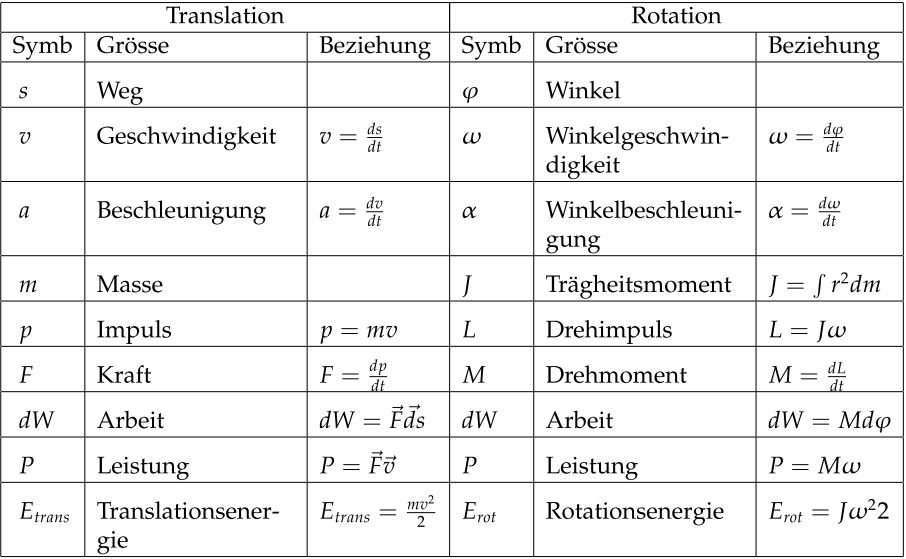
\includegraphics{bilder/trans-rotation}}
%Dynamik
\newpage
\section{Dynamik}
\subsection{Newtonsche Gesetze}
\subsubsection{Erstes Newtonsches Gesetz Trägheitsgesetz}
Ein Körper verharrt im Zustand der Ruhe oder der gleichförmigen Bewegung, wenn er
nicht durch einwirkende Kräfte gezwungen wird, seinen Zustand zu ändern. Die Gesamt-
summe der Kräfte in einem abgeschlossenen System ist unveränderlich:

\subsubsection{Zweites Newtonsches Gesetz (Aktionsgesetz)}
Die Beschleunigung eines Körpers ist umgekehrt proportional zu seiner Masse und direkt
proportional zur Kraft, die auf ihn wirkt.

\subsubsection{Drittes Newtonsches Gesetz (Actio = Reactio)}
Wirkt ein Körper A auf einen Körper B mit der Kraft ~F AB , so wirkt der Körper B mit der
entgegengesetzt gerichteten, gleich grossen Kraft $\overrightarrow{F}_{BA}$.

\subsubsection{Allgemeines Vorgehen beim Lösen von Bewegungsproblemen}
\begin{enumerate}
	\item Zeichnung anfertigen
	\item Für jeden Körper, der untersucht werden soll, wird ein Kräftediagramm eingezeichnet
	\item Ein geeignetes Koordinatensystem einführen
	\item  Das entstandene Gleichungssystem aufl"osen
	\item  Ergebnisse mit gesundem Menschenverstand aufl"osen
\end{enumerate}

$F_{G} = Gewichtskraft$
$F_{R} = Reibungskraft$
$F_{N} = Normalkraft$
$\mu_{G} = Gleitreibung$
$\mu_{H} = Haftreibung$
$W_{B} = Beschleunigungsarbeit$
$E_{kin} = Kinetische Energie$

\subsubsection{Spezielle Kräfte, Masse, Dichte, Reibung}
$F_{G} = mg$ \\
$F_{R} = \mu_{G}F_{N}$ \\
$\rho = \frac{m}{V}$ \\
$\mu = - \frac{a}{g}$ \\
$\mu_{H} = \tan{}$ \\
$F_{H_{max}} = \mu_{H}F_{H}$ \\ 

\subsubsection{Arbeit und Energie, Energieerhaltung}
Energie ist die Fähigkeit Arbeit zu leisten. Arbeit = überwinden eines Widerstandes \\
Energie kann weder verschwinden, noch aus dem Nichts entstehen. 
Wenn gelegentlich davon gesprochen wird, dass Energie 
”vernichtet“ werde, so ist damit gemeint, dass mechanische Energie 
(potentielle oder kinetische Energie) durch Reibungsarbeit in 
”Wärme“, genauer gesagt, in innere Energie, umgewandelt wird. \\
Die Gesamtenergie eines abgeschlossenen Systems ist 
unveränderlich. \\
$dW = \overrightarrow{F} \cdot \overrightarrow{ds}$
$W = Pt$
$F = \frac{P}{v}$

\subsubsection{Leistung}

$P = \frac{\Delta W}{\Delta t} = \frac{\overrightarrow{F} \Delta \overrightarrow{s}}{ \Delta t} = \overrightarrow{F} \cdot \frac{\Delta \overrightarrow{s}}{\Delta t} = \overrightarrow{F} \cdot \overrightarrow{v} = \overrightarrow{M} \cdot \omega$ \\
Umwandlung von $1 kWh = 3.6 \cdot 10^3 J $ (Überprüfen) \\
1 PS = 735.5 W


\subsubsection{Hubarbeit, Potentielle Energie}

Potentielle Energie $E_{pot} = m \cdot g \cdot h$ \\
$W_{H} \cdot \overrightarrow{F} \cdot \overrightarrow{h}$ \\
Hubarbeit: $W_{H} = E_{pot}$

\subsubsection{Spannarbeit, Spannenergie}
Spannenergie: $E_{s} = \frac{c \cdot x^2}{2}$  entspricht Spannarbeit: $W_{s} = \overrightarrow{F_{s}} \cdot \overrightarrow{x}$ \\
x: = Spannweg [m], $F_{s}$ = Spannkraft


\subsubsection{Beschleunigungsarbeit, Kinetische Energie}
$E_{kin} = \frac{mv^2}{2}$
$W_{B} = \frac{m(\Delta v)^2}{2}$

\subsubsection{Rotationsenergie}
$E_{rot} = \frac{1}{2}Jw^2$

\subsubsection{Reibungsarbeit}
$W_{R} = F_{RS}$

\subsubsection{Verformungsarbeit}
$Inelatisch: W_{D} = \frac{m_{1}m_{2}(v_{1} + v_{2})^2}{2(m_{1} + m_{2})} $ \\
$Elatisch:  W_{D} = \frac{F_{1} + F_{2}}{2}\Delta s$

\subsubsection{Kernbindungenergie (Einstein)}
$E = m \cdot c^2$

\subsubsection{Leistung}
$P = \frac{dW}{dt} = \frac{Fds}{dt} =\overrightarrow{F} \cdot \overrightarrow{s} = M \cdot \omega$

\subsubsection{Wirkungsgrad}
Beachte: Wo wird die Systemgrenze gezogen?! Wird z.B. die Wärmeleistung weiterverwendet? \\
Wirkungsgrad: $\eta = \frac{P_{ab}}{P_{zu}} = \frac{W_{ab}}{W_{zu}}$ \\
$\eta_{tot} = \eta_{1} \cdot \eta_{2}  \cdot ...$

\subsubsection{Impuls, Impulserhaltung}
Impuls $ \overrightarrow{p} = m \cdot \overrightarrow{v} = \overrightarrow{F}$  \\
Gesamtimpuls: $ p_{ges} = \Sigma_{i = 1} m_{i}v_{s} $\\
Kraftstoss: $\overrightarrow{F} = \frac{\Delta \overrightarrow{p}}{ \Delta t}$

\subsubsection{Drehimpuls}
Drehimpuls: $L = m \cdot v \cdot r \cdot \sin{\phi} = J \cdot \omega$ \\
$\overrightarrow{L} = \overrightarrow{r} \times \overrightarrow{p}$ \\
Drehmoment: $ \overrightarrow{M} = \frac{d \overrightarrow{p}}{dt}
$

\subsubsection{Raketenantrieb}

\subsubsection{Inelastischer Stoss}

\subsubsection{Elastischer Stoss}





% Wichtige allgemeine Formeln
\subsection{Dreiecksformeln}
\begin{tabular}{lll}
	& \parbox{9.5cm}{
		\textbf{Cosinussatz} \\
		$$c^2 = a^2 + b^2 - 2 \cdot a \cdot b \cdot \cos \gamma$$\\
		\textbf{Sinussatz} \\
		$$\frac{a}{\sin \alpha} = \frac{b}{\sin \beta} = \frac{c}{\sin \gamma} = 2r =
		\frac{u}{\pi}$$
		\textbf{Pythagoras beim Sinus}\\
		$$\sin^2(b)+\cos^2(b)=1 \qquad \tan(b)=\frac{\sin(b)}{\cos(b)}$$}
		
	& \parbox{8cm}{
		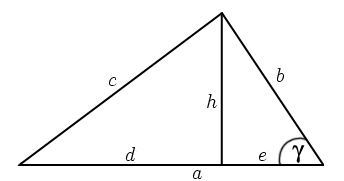
\includegraphics[width=6cm]{./idiotenseite/images/cosinussatz.png}}
\end{tabular}
\begin{center}
	\begin{multicols}{2}
		$\sin \beta = \frac ba =\frac{\text{Gegenkathete}}{\text{Hypotenuse}}$\\
		$\cos \beta = \frac ca =\frac{\text{Ankathete}}{\text{Hypotenuse}}$\\
		$\tan \beta = \frac cb =\frac{\text{Gegenkathete}}{\text{Ankathete}}$\\
		$\cot \beta = \frac cb =\frac{\text{Ankathete}}{\text{Gegenkathete}}$\\
	\end{multicols}
\end{center}

	
\subsection{Funktionswerte für Winkelargumente}
	\begin{multicols}{4}	
	\begin{tabular}[c]{|p{0.5cm}|p{0.4cm}||p{0.5cm}|p{0.5cm}|p{0.5cm}|}
	    	\hline
			deg & rad & sin & cos & tan\\
			\hline
			0\symbol{23} & 0 & 0 & 1 & 0\\
			\hline
			30\symbol{23} & $\frac{\pi}{6}$ & $\frac{1}{2}$ & $\frac{\sqrt{3}}{2}$ &
			$\frac{\sqrt{3}}{3}$\\
			\hline
			45\symbol{23} & $\frac{\pi}{4}$ & $\frac{\sqrt{2}}{2}$ & $\frac{\sqrt{2}}{2}$
			& 1\\
			\hline
			60\symbol{23} & $\frac{\pi}{3}$ & $\frac{\sqrt{3}}{2}$ & $\frac{1}{2}$ &
			$\sqrt{3}$\\
			\hline			
	\end{tabular} \\
	
	\begin{tabular}[c]{|p{0.7cm}|p{0.7cm}||p{0.7cm}|p{0.7cm}|}
	    	\hline
			deg & rad & sin & cos\\
			\hline
			90\symbol{23} & $\frac{\pi}{2}$ & 1 & 0\\
			\hline	
			120\symbol{23} & $\frac{2\pi}{3}$ & $\frac{\sqrt{3}}{2}$ & $-\frac{1}{2}$ \\
			\hline
			135\symbol{23} & $\frac{3\pi}{4}$ & $\frac{\sqrt{2}}{2}$ & $-\frac{\sqrt{2}}{2}$\\
			\hline
			150\symbol{23} & $\frac{5\pi}{6}$ & $\frac{1}{2}$ & $-\frac{\sqrt{3}}{2}$\\
			\hline
	\end{tabular} \\
	
	\begin{tabular}[c]{|p{0.7cm}|p{0.7cm}||p{0.7cm}|p{0.7cm}|}
	  	\hline
		deg & rad & sin & cos\\
		\hline
		180\symbol{23} & $\pi$ & 0 & -1\\
		\hline	
		210\symbol{23} & $\frac{7\pi}{6}$ & $-\frac{1}{2}$ & $-\frac{\sqrt{3}}{2}$\\
		\hline
		225\symbol{23} & $\frac{5\pi}{4}$ & $-\frac{\sqrt{2}}{2}$ & $-\frac{\sqrt{2}}{2}$\\
		\hline
		240\symbol{23} & $\frac{4\pi}{3}$ & $-\frac{\sqrt{3}}{2}$ & $-\frac{1}{2}$\\
		\hline
	\end{tabular} \\
	
	\begin{tabular}[c]{|p{0.7cm}|p{0.7cm}||p{0.7cm}|p{0.7cm}|}
    	\hline
		deg & rad & sin & cos\\
		\hline
		270\symbol{23} & $\frac{3\pi}{2}$ & -1 & 0\\
		\hline	
		300\symbol{23} & $\frac{5\pi}{3}$ & $-\frac{\sqrt{3}}{2}$ & $\frac{1}{2}$\\
		\hline
		315\symbol{23} & $\frac{7\pi}{4}$ & $-\frac{\sqrt{2}}{2}$ & $\frac{\sqrt{2}}{2}$\\
		\hline
		330\symbol{23} & $\frac{11\pi}{6}$ & $-\frac{1}{2}$ & $\frac{\sqrt{3}}{2}$\\
		\hline
	\end{tabular}					
\end{multicols}

\begin{minipage}{13cm}
	\subsection{Periodizität}
	$\cos(a+k\cdot2\pi)=\cos(a) \qquad \sin(a+k\cdot2\pi)=\sin(a) \qquad
	(k \in \mathbb{Z})$
	\subsection{Quadrantenbeziehungen}
	\begin{tabbing}
    	xxxxxxxxxxxxxxxxxxxxxxxxxxxxxxxxxx \= \kill
	  	$\sin(-a)=-\sin(a)$ \> $\cos(-a)=\cos(a)$\\
		$\sin(\pi - a)=\sin(a)$ \> $\cos(\pi - a)=-\cos(a)$\\
		$\sin(\pi + a)=-\sin(a)$ \> $\cos(\pi +a)=-\cos(a)$\\
		$\sin\left(\frac{\pi}{2}-a \right)=\sin\left(\frac{\pi}{2}+a \right)=\cos(a)$ \>
		$\cos\left(\frac{\pi}{2}-a \right)=-\cos\left(\frac{\pi}{2}+a \right)=\sin(a)$  
    \end{tabbing}
\end{minipage}
\begin{minipage}{5cm}
	

\subsection{Ableitungen}

\begin{tikzpicture}
	[	inner sep = 2mm,
		sin/.style={rectangle,minimum width=1.2cm,minimum height=1cm,rounded corners=5pt,draw=black,top color=green!20!black!50},
		abl/.style={rectangle}
	]
	\node at (1.2,0) (sin1) [sin] {$\sin$};
	\node at (0,-1.2) (cos2) [sin] {$-\cos$};
	\node at (1.2,-2.4) (sin2) [sin] {$-\sin$};
	\node at (2.4,-1.2) (cos1) [sin] {$\cos$};
	
	\draw[thick,black,->] (sin1.east) .. controls +(right:0.6cm) and +(up:0.6cm) ..  (cos1.north)
	node [pos=0.5,above](abl) {$\frac{d}{dx}$};
	\draw[thick,black,->] (cos1.south) .. controls +(down:0.6cm) and +(right:0.6cm) .. (sin2.east)
	node [pos=0.5,below](abl) {$\frac{d}{dx}$};
	\draw[thick,black,->] (sin2.west) .. controls +(left:0.6cm) and +(down:0.6cm) .. (cos2.south)
	node [pos=0.5,below](abl) {$\frac{d}{dx}$};
	\draw[thick,black,->] (cos2.north) .. controls +(up:0.6cm) and +(left:0.6cm) .. (sin1.west)
	node [pos=0.5,above](abl) {$\frac{d}{dx}$};
\end{tikzpicture}
\end{minipage}
\begin{multicols}{2}
	\subsection{Additionstheoreme}
	$\sin(a \pm b)=\sin(a) \cdot \cos(b) \pm \cos(a) \cdot \sin(b)$\\
	$\cos(a \pm b)=\cos(a) \cdot \cos(b) \mp \sin(a) \cdot \sin(b)$\\	
	$\tan(a \pm b)=\dfrac{\tan(a) \pm \tan(b)}{1 \mp \tan(a) \cdot \tan(b)}$
	\columnbreak
	
	\subsection{Doppel- und Halbwinkel}	
	$\sin(2a)=2\sin(a)\cos(a)$\\
	$\cos(2a)=\cos^2(a)-\sin^2(a)=2\cos^2(a)-1=1-2\sin^2(a)$\\
	$\cos^2 \left(\frac{a}{2}\right)=\frac{1+\cos(a)}{2} \qquad
	\sin^2 \left(\dfrac{a}{2}\right)=\frac{1-\cos(a)}{2}$
\end{multicols}
\begin{multicols}{2}
	\subsection{Produkte}
		$\sin(a)\sin(b)=\frac{1}{2}(\cos(a-b)-\cos(a+b))$\\
		$\cos(a)\cos(b)=\frac{1}{2}(\cos(a-b)+\cos(a+b))$\\
		$\sin(a)\cos(b)=\frac{1}{2}(\sin(a-b)+\sin(a+b))$\\
	\subsection{Euler-Formeln} 

	$\sin(x) = \frac{1}{2j} \left(e^{jx} - e^{-jx}\right) \qquad
	\cos(x) = \frac{1}{2} \left(e^{jx} + e^{-jx}\right)$ \\
	$e^{x+jy} = e^x \cdot e^{jy} = e^x \cdot \left(\cos(y) + j\sin(y)\right)$ \\
	$e^{j\pi} = e^{-j\pi} = -1$ \\
	\columnbreak
	
	\subsection{Summe und Differenz}
		$\sin(a)+\sin(b)=2 \cdot \sin \left(\frac{a+b}{2}\right) \cdot
		\cos\left(\frac{a-b}{2}\right)$\\
		$\sin(a)-\sin(b)=2 \cdot \sin \left(\frac{a-b}{2}\right) \cdot
		\cos\left(\frac{a+b}{2}\right)$\\
		$\cos(a)+\cos(b)=2 \cdot \cos \left(\frac{a+b}{2}\right) \cdot
		\cos\left(\frac{a-b}{2}\right)$\\
		$\cos(a)-\cos(b)=-2 \cdot \sin \left(\frac{a+b}{2}\right) \cdot
		\sin\left(\frac{a-b}{2}\right)$\\
		$\tan(a) \pm \tan(b)=\dfrac{\sin(a \pm b)}{\cos(a)\cos(b)}$\\
\end{multicols}

%\input{idiotenseite/trigo/Fragen}


\end{document}